\documentclass[11pt]{article}

\usepackage[margin=1in]{geometry}
\usepackage{amsmath,amssymb,amsthm,mathtools,bm}
\usepackage{booktabs}
\usepackage{graphicx}
\usepackage{xcolor}
\usepackage{caption}
\usepackage{enumitem}
\usepackage[colorlinks=true,linkcolor=blue!55!black,citecolor=blue!55!black,urlcolor=blue!55!black]{hyperref}
\usepackage{microtype}

\graphicspath{{../analysis/}}

\newcommand{\passk}[1]{\ensuremath{\mathrm{pass}@#1}}
\newcommand{\Rout}{\ensuremath{R_{\mathrm{out}}}}
\newcommand{\Rpv}{\ensuremath{R_{\mathrm{pv}}}}
\newcommand{\ind}[1]{\ensuremath{\mathbb{1}\!\left[#1\right]}}
\newcommand{\pp}{\,\mathrm{pp}}
\newcommand{\ci}[2]{\ensuremath{[#1,\,#2]}}

\title{\textbf{Experiment 4 — Process-Aware Rewards and Reward Hacking}\\[4pt]
\large A Validated Replication of \S6 (Figs.\ 7--8) of Zhang, Neubig \& Yue (2025)}
\author{DLT Final Project — Experiment 4\\[2pt]
\small PACE ICE, $1\times$ H100 (job 6589709), 1\,h\,20\,m, 640{,}000 sampled solutions}
\date{October 2026}

\begin{document}
\maketitle

\begin{abstract}
We replicate \S6 of \emph{On the Interplay of Pre-Training, Mid-Training, and RL on
Reasoning Language Models} (arXiv 2512.07783, ICML 2026 Spotlight) on the authors'
released checkpoints: one shared 100M-parameter base model and four GRPO runs differing
\emph{only} in reward composition (outcome-only, two mixes, and a strict process gate),
evaluated with $k{=}64$ samples on $2{,}000$ problems in two contexts ($640$k samples).
The paper's central claim is confirmed, and decisively: the \textbf{reward-hacking rate}
--- the share of correct answers reached through invalid reasoning --- falls
monotonically with process-supervision strength on the long-tail context
($52.3\% \to 45.8\% \to {\approx}42.3\% \to 40.5\%$), with \emph{every} step of the
ladder significant under paired bootstrap after Bonferroni correction (strict vs.\
outcome: $-5.31\pp$, \ci{-6.37}{-4.27}). Strict \passk{1} gains from process rewards
are decisive on edge-difficulty problems ($+6.5\pp$, \ci{+2.8}{+10.3}) and directional
but individually unresolved on the hardest band. All numbers are reproduced from the
raw samples and validated by four independent audits.
\end{abstract}

\section{Question and systems}

\paragraph{Question.} Compared with an \emph{outcome-only} reward (pay for the correct
final answer), do \emph{mixed} or \emph{strict process} rewards (also pay for verified
reasoning steps) (a) raise strict \passk{k} and (b) lower the reward-hacking rate?

\paragraph{Five systems.} One 100M-parameter base model (pre-trained $99.9\%$
\texttt{crazy\_zootopia} at $\mathrm{op}\,2$--$20$ $+\,0.1\%$ \texttt{teachers\_in\_school}
at $\mathrm{op}\,2$--$20$; the paper's appendix A.6.1 ``shared primitives'' setting) and
four GRPO runs from it on \emph{identical} data ($90\%$ zoo / $10\%$ teachers,
$\mathrm{op}\,2$--$20$, $204{,}800$ samples $\approx 200$ steps), differing only in
reward:

\begin{table}[h]\centering\small
\begin{tabular}{lll}
\toprule
Label & Reward (verified from released configs) & Status \\
\midrule
\texttt{base} & none (pre-training only) & --- \\
\texttt{outcome} & $R = \ind{\hat a = a^{*}}$ (pure answer match) & verified \\
\texttt{0.5/0.5} & $R = \ind{\hat a = a^{*}}\cdot(0.5 + 0.5\,\Rpv)$ & weights assumed \\
\texttt{0.2/0.8} & $R = \ind{\hat a = a^{*}}\cdot(0.2 + 0.8\,\Rpv)$ & verified \\
\texttt{strict} & $R = \ind{\hat a = a^{*}}\cdot\ind{\Rpv = 1}$ & verified \\
\bottomrule
\end{tabular}
\end{table}

\noindent Here $\Rpv$ is the \emph{process accuracy} --- the fraction of gold
reasoning-graph nodes the solution reproduces with correct parents and values. The
released code applies an \emph{answer gate} (reward zeroed when the answer is wrong), so
the mixes are conditional on a correct answer; this diverges from the paper's literal
Eq.~3, which was never trained in the released family.

\section{Method}

\begin{table}[h]\centering\small
\begin{tabular}{ll}
\toprule
Choice & Value \\
\midrule
Eval data & \texttt{crazy\_zootopia} + \texttt{teachers\_in\_school} val, $\mathrm{op}\in\{12,14,16,18,20\}$, 200/op \\
Samples & $k=64$/problem, temperature $0.7$, top-$p$ $1.0$, $\le 1024$ new tokens \\
Budget & $5 \times 2 \times 1{,}000 \times 64 = 640{,}000$ samples \\
Scoring & authors' graph pipeline: strict (process-verified) + answer-only \passk{k} \\
Bands & edge $=\mathrm{op}\,12$--$14$, hard $=\mathrm{op}\,16$--$20$ \\
Uncertainty & bootstrap over problems ($B{=}1000$); \textbf{paired} bootstrap for contrasts ($B{=}5000$); Bonferroni $\alpha{=}0.05/9$ \\
\bottomrule
\end{tabular}
\end{table}

\paragraph{Metrics.} With first-success rank $r_i$ of problem $i$,
$\passk{k} = \tfrac{1}{N}\sum_i \ind{r_i < k}$. With $a_i$ answer-correct and $s_i$
strictly-correct samples (of 64),
\[ H \;=\; \frac{\sum_i \max(0, a_i - s_i)}{\sum_i a_i}
\;=\; \Pr\big(\text{invalid reasoning} \mid \text{correct answer}\big). \]

\section{Results}

\subsection{Headline --- both contexts, overall}

\begin{table}[h]\centering\small
\caption{Strict and answer-only \passk{k}, and hacking rate (\%), overall. Hacking CIs
are $95\%$ bootstrap over problems.}
\begin{tabular}{llccccc}
\toprule
Context & Reward & strict @1 & strict @64 & ans @1 & ans @64 & hacking rate \\
\midrule
\multirow{5}{*}{teachers}
 & base    & 20.3 & 62.7 & 42.7 & 95.2 & \textbf{52.3} \ci{49.1}{55.7} \\
 & outcome & 36.1 & 68.8 & 66.9 & 94.4 & \textbf{45.8} \ci{42.7}{48.8} \\
 & 0.5/0.5 & 40.0 & 70.3 & 69.5 & 93.9 & \textbf{42.3} \ci{39.3}{45.7} \\
 & 0.2/0.8 & 39.2 & 68.0 & 68.6 & 93.4 & \textbf{42.2} \ci{38.7}{45.4} \\
 & strict  & 38.7 & 68.8 & 64.4 & 94.4 & \textbf{40.5} \ci{37.3}{43.5} \\
\midrule
\multirow{5}{*}{zoo}
 & base    & 60.3 & 87.0 & 89.5 & 99.6 & 33.6 \ci{30.9}{36.6} \\
 & outcome & 64.3 & 85.1 & 92.8 & 98.7 & 32.6 \ci{29.8}{35.3} \\
 & 0.5/0.5 & 62.3 & 86.4 & 92.7 & 98.7 & 32.3 \ci{29.6}{34.9} \\
 & 0.2/0.8 & 62.6 & 86.2 & 93.0 & 98.6 & 32.2 \ci{29.5}{34.9} \\
 & strict  & 63.0 & 85.6 & 92.5 & 98.9 & 32.0 \ci{29.2}{34.8} \\
\bottomrule
\end{tabular}
\end{table}

\subsection{The reward-hacking ladder (teachers) --- the strongest result}

Hacking falls monotonically with process-supervision strength. Because all five
checkpoints answered \emph{identical} problems, the right test is the paired bootstrap;
\textbf{every step of the ladder is significant and survives Bonferroni} ($^{\dagger}$).

\begin{table}[h]\centering\small
\begin{tabular}{lcc}
\toprule
Paired contrast (teachers, overall) & $\Delta$ hacking (pp) & $95\%$ CI \\
\midrule
base $-$ outcome    & $+6.51$ & \ci{+4.74}{+8.25}$^{\dagger}$ \\
0.5/0.5 $-$ outcome & $-3.48$ & \ci{-4.35}{-2.62}$^{\dagger}$ \\
0.2/0.8 $-$ outcome & $-3.59$ & \ci{-4.46}{-2.73}$^{\dagger}$ \\
\textbf{strict} $-$ outcome & $\bm{-5.31}$ & \ci{-6.37}{-4.27}$^{\dagger}$ \\
\bottomrule
\end{tabular}
\end{table}

\subsection{Strict \texorpdfstring{\passk{k}}{pass@k} by difficulty band}

\begin{table}[h]\centering\small
\begin{tabular}{llccccc}
\toprule
Context & Band / metric & base & outcome & 0.5/0.5 & 0.2/0.8 & strict \\
\midrule
teachers & edge \passk{1}  & 33.5 & 44.8 & \textbf{51.2} & 47.8 & 48.0 \\
teachers & edge \passk{64} & 80.8 & 81.0 & 81.5 & 80.5 & \textbf{83.0} \\
teachers & hard \passk{1}  & 11.5 & 30.3 & 32.5 & \textbf{33.5} & 32.5 \\
teachers & hard \passk{64} & 50.7 & 60.7 & \textbf{62.8} & 59.7 & 59.3 \\
zoo & edge \passk{1}  & 68.8 & 71.0 & 67.8 & 68.2 & 69.8 \\
zoo & edge \passk{64} & \textbf{94.5} & 89.8 & 92.8 & 92.2 & 93.2 \\
zoo & hard \passk{1}  & 54.7 & 59.8 & 58.7 & 58.8 & 58.5 \\
zoo & hard \passk{64} & 82.0 & 82.0 & \textbf{82.2} & 82.2 & 80.5 \\
\bottomrule
\end{tabular}
\end{table}

\noindent Key paired contrasts:
\begin{itemize}[leftmargin=1.4em,itemsep=1pt]
\item \textbf{RL vs.\ base (teachers):} hard \passk{1} $+18.8\pp$ \ci{+15.2}{+22.5};
hard \passk{64} $+10.0\pp$ \ci{+6.7}{+13.3}.
\item \textbf{Process vs.\ outcome, edge:} $0.5/0.5 - \text{outcome} = +6.50\pp$
\ci{+2.75}{+10.25} (Bonferroni-robust).
\item \textbf{Process vs.\ outcome, hard:} all three ahead ($+2.2$ to $+3.2\pp$),
sign-consistent across all 5 ops (sign test $p=0.031$), but none individually excludes
zero (best $p=0.056$) --- directional support.
\item \textbf{Zoo edge \passk{64}:} base $-$ outcome $= +4.75\pp$ \ci{+2.25}{+7.25} ---
RL narrows the sampled solution set where the base was already strong.
\end{itemize}

\subsection{Per-op strict \texorpdfstring{\passk{1}}{pass@1} (teachers)}

\begin{table}[h]\centering\small
\begin{tabular}{lccccc}
\toprule
Reward & op 12 & op 14 & op 16 & op 18 & op 20 \\
\midrule
base    & 43.5 & 23.5 & 12.0 & 14.0 & 8.5 \\
outcome & 51.5 & 38.0 & 34.5 & 30.5 & 26.0 \\
0.5/0.5 & 57.0 & 45.5 & 34.5 & 36.5 & 26.5 \\
0.2/0.8 & 52.0 & 43.5 & 35.5 & 37.0 & 28.0 \\
strict  & 53.5 & 42.5 & 37.5 & 33.0 & 27.0 \\
\bottomrule
\end{tabular}
\end{table}

\noindent Process variants beat outcome-only in 14 of 15 (op $\times$ variant) cells
and tie once --- the sign-consistency behind the hard-band sign test.

\subsection{Error breakdown (teachers, share of all samples \%)}

\begin{table}[h]\centering\small
\caption{Hard band (op 16--20).}
\begin{tabular}{lccccc}
\toprule
Reward & correct & wrong dep.\ & missing steps & wrong value & wrong answer \\
\midrule
base    & 11.7 & 86.5 & 46.6 & 79.3 & 69.2 \\
outcome & 29.5 & 68.1 & 30.1 & 47.8 & 40.5 \\
0.5/0.5 & 32.0 & 66.7 & \textbf{24.8} & 47.8 & 40.0 \\
0.2/0.8 & 32.0 & 66.8 & 27.6 & 48.2 & 40.5 \\
strict  & 30.9 & 67.9 & \emph{34.7} & 52.0 & 44.5 \\
\bottomrule
\end{tabular}
\end{table}

\begin{table}[h]\centering\small
\caption{Edge band (op 12--14).}
\begin{tabular}{lccccc}
\toprule
Reward & correct & wrong dep.\ & missing steps & wrong value & wrong answer \\
\midrule
base    & 32.3 & 63.8 & 20.4 & 48.4 & 41.7 \\
outcome & 46.3 & 50.8 & 16.1 & 27.7 & 22.3 \\
0.5/0.5 & 49.6 & 48.3 & \textbf{11.9} & 26.5 & 20.7 \\
0.2/0.8 & 48.9 & 49.2 & 13.5 & 27.2 & 21.4 \\
strict  & 49.2 & 48.8 & 14.6 & 27.9 & 22.6 \\
\bottomrule
\end{tabular}
\end{table}

\noindent Process rewards shift errors away from structural failures, the dense mixes
most clearly. \emph{Nuance:} strict gating \emph{increases} missing-step errors on the
hard band ($34.7\%$ vs.\ outcome's $30.1\%$) while dense mixes decrease them
($\to 24.8\%$) --- an all-or-nothing trace reward favors short, conservative
derivations; a dense per-step reward pays for completing each step.

\begin{figure}[t]\centering
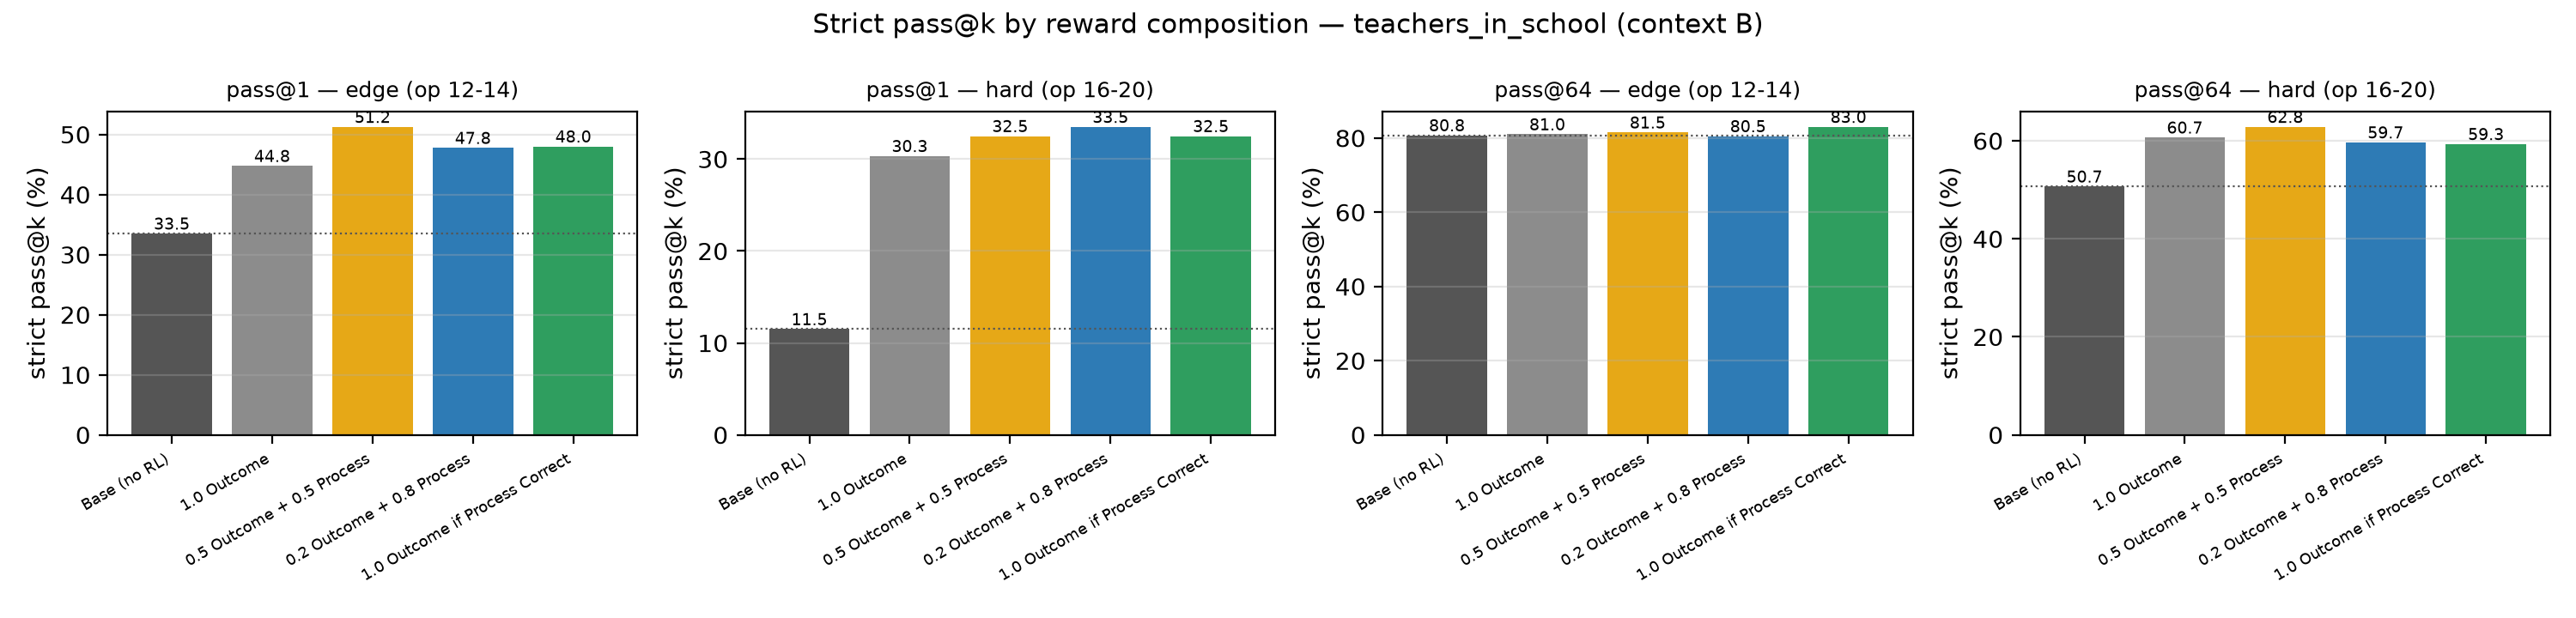
\includegraphics[width=.92\linewidth]{fig7_bars_teachers.png}
\caption{Strict \passk{1}/\passk{64} by reward composition and band, teachers context.}
\end{figure}

\begin{figure}[t]\centering
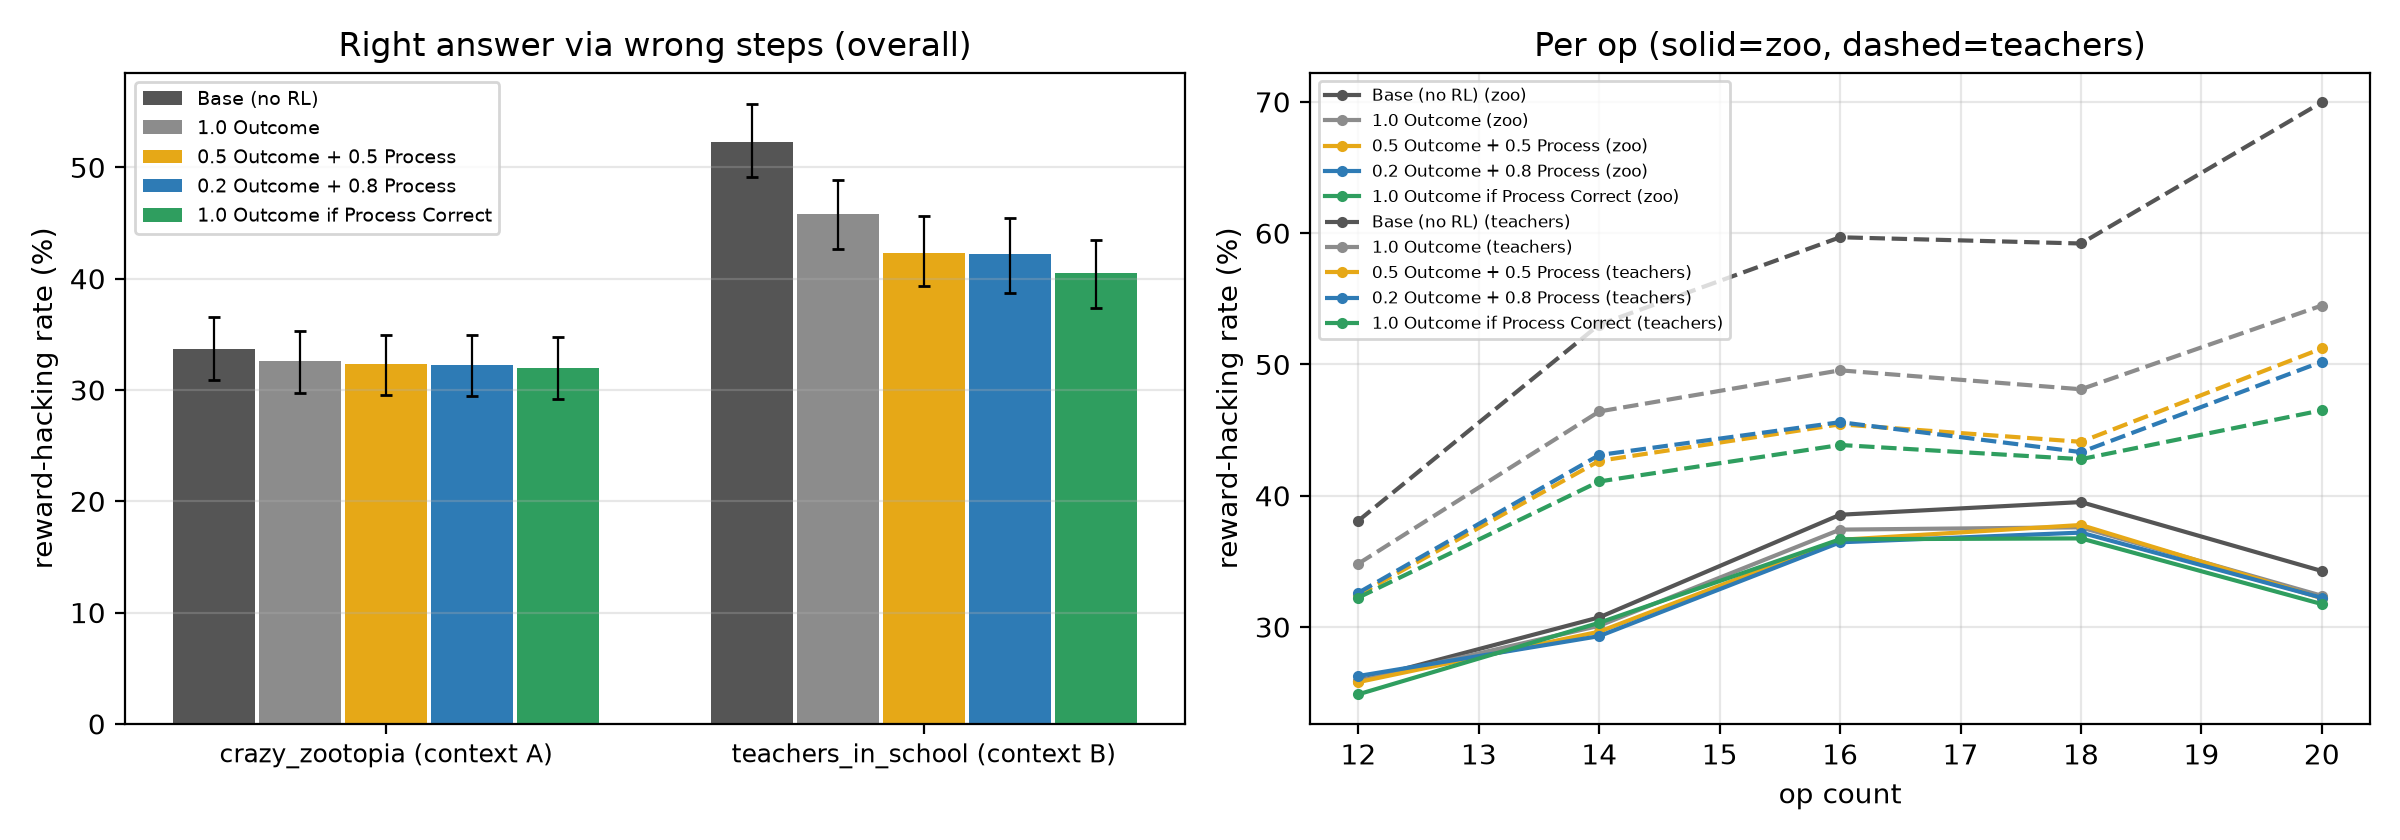
\includegraphics[width=.92\linewidth]{fig_hacking_rate.png}
\caption{Reward-hacking rate by reward composition: overall per context (left, with
$95\%$ CIs) and per op count (right).}
\end{figure}

\section{Verdicts vs.\ the paper's predictions}
\begin{enumerate}[leftmargin=1.6em,itemsep=1pt]
\item \emph{``Process signal raises strict \passk{1} by ${\sim}4$--$5$ pp on the hardest
problems.''} --- \textbf{Directional} on hard ($+2.2$ to $+3.2\pp$, sign-consistent,
individually unresolved); \textbf{unambiguous on edge} ($+6.5\pp$ \ci{+2.8}{+10.3}).
\item \emph{``0.2/0.8 and strict best; strict lowest hacking.''} --- \textbf{Confirmed};
the hacking ladder is Bonferroni-robust at every step.
\item \emph{``Errors shift away from wrong dependencies and missing steps.''} ---
\textbf{Supported}, with the strict-gating missing-step reversal as a refinement.
\end{enumerate}

\section{Validation and limitations}
Four audits: data integrity (all $64{,}000$-record runs complete, byte-identical
problems across checkpoints, zero truncation/duplicates); clean-room recomputation
(independent code matching these numbers to ${\sim}10^{-16}$ and the authors' aggregator
exactly); qualitative re-scoring ($240/240$); paired statistics (CIs ${\sim}3\times$
tighter than independent via shared-difficulty cancellation).

\noindent\textbf{Limitations.} One training run per reward (CIs cover evaluation
uncertainty only); context-setting substitution (direction-comparable to the paper's
extrapolation-setting \S6, not number-comparable); $k{=}64$ not $128$; the $0.5/0.5$
weights assumed. A letter-collision artifact in the authors' strict scorer inflates
\emph{absolute} hacking rates and deflates \emph{absolute} strict \passk{k} for all
checkpoints equally; the \emph{paired differences and orderings} reported here are
robust, but absolute levels should not be compared literally against the paper.

\section{Reproducibility}
One command on PACE: \texttt{sbatch scripts/run\_all\_pace.sbatch} (pinned: vLLM
$0.10.1.1$, transformers $4.55.2$, torch $2.7.1$). Pipeline: HF downloads
$\to$ smoke test $\to$ vLLM generation $\to$ graph scoring $\to$ analysis
(\texttt{src/analyze\_e4.py}, bootstrap seed 0; paired bootstrap seed 12345)
$\to$ figures. Raw samples in \texttt{results/}; metrics, CSVs, figures, and the
four-audit validation in \texttt{analysis/}. Total compute: $1$\,h\,$20$\,m on one H100.

\clearpage
\appendix
\section{Additional figures}

\begin{figure}[h]\centering
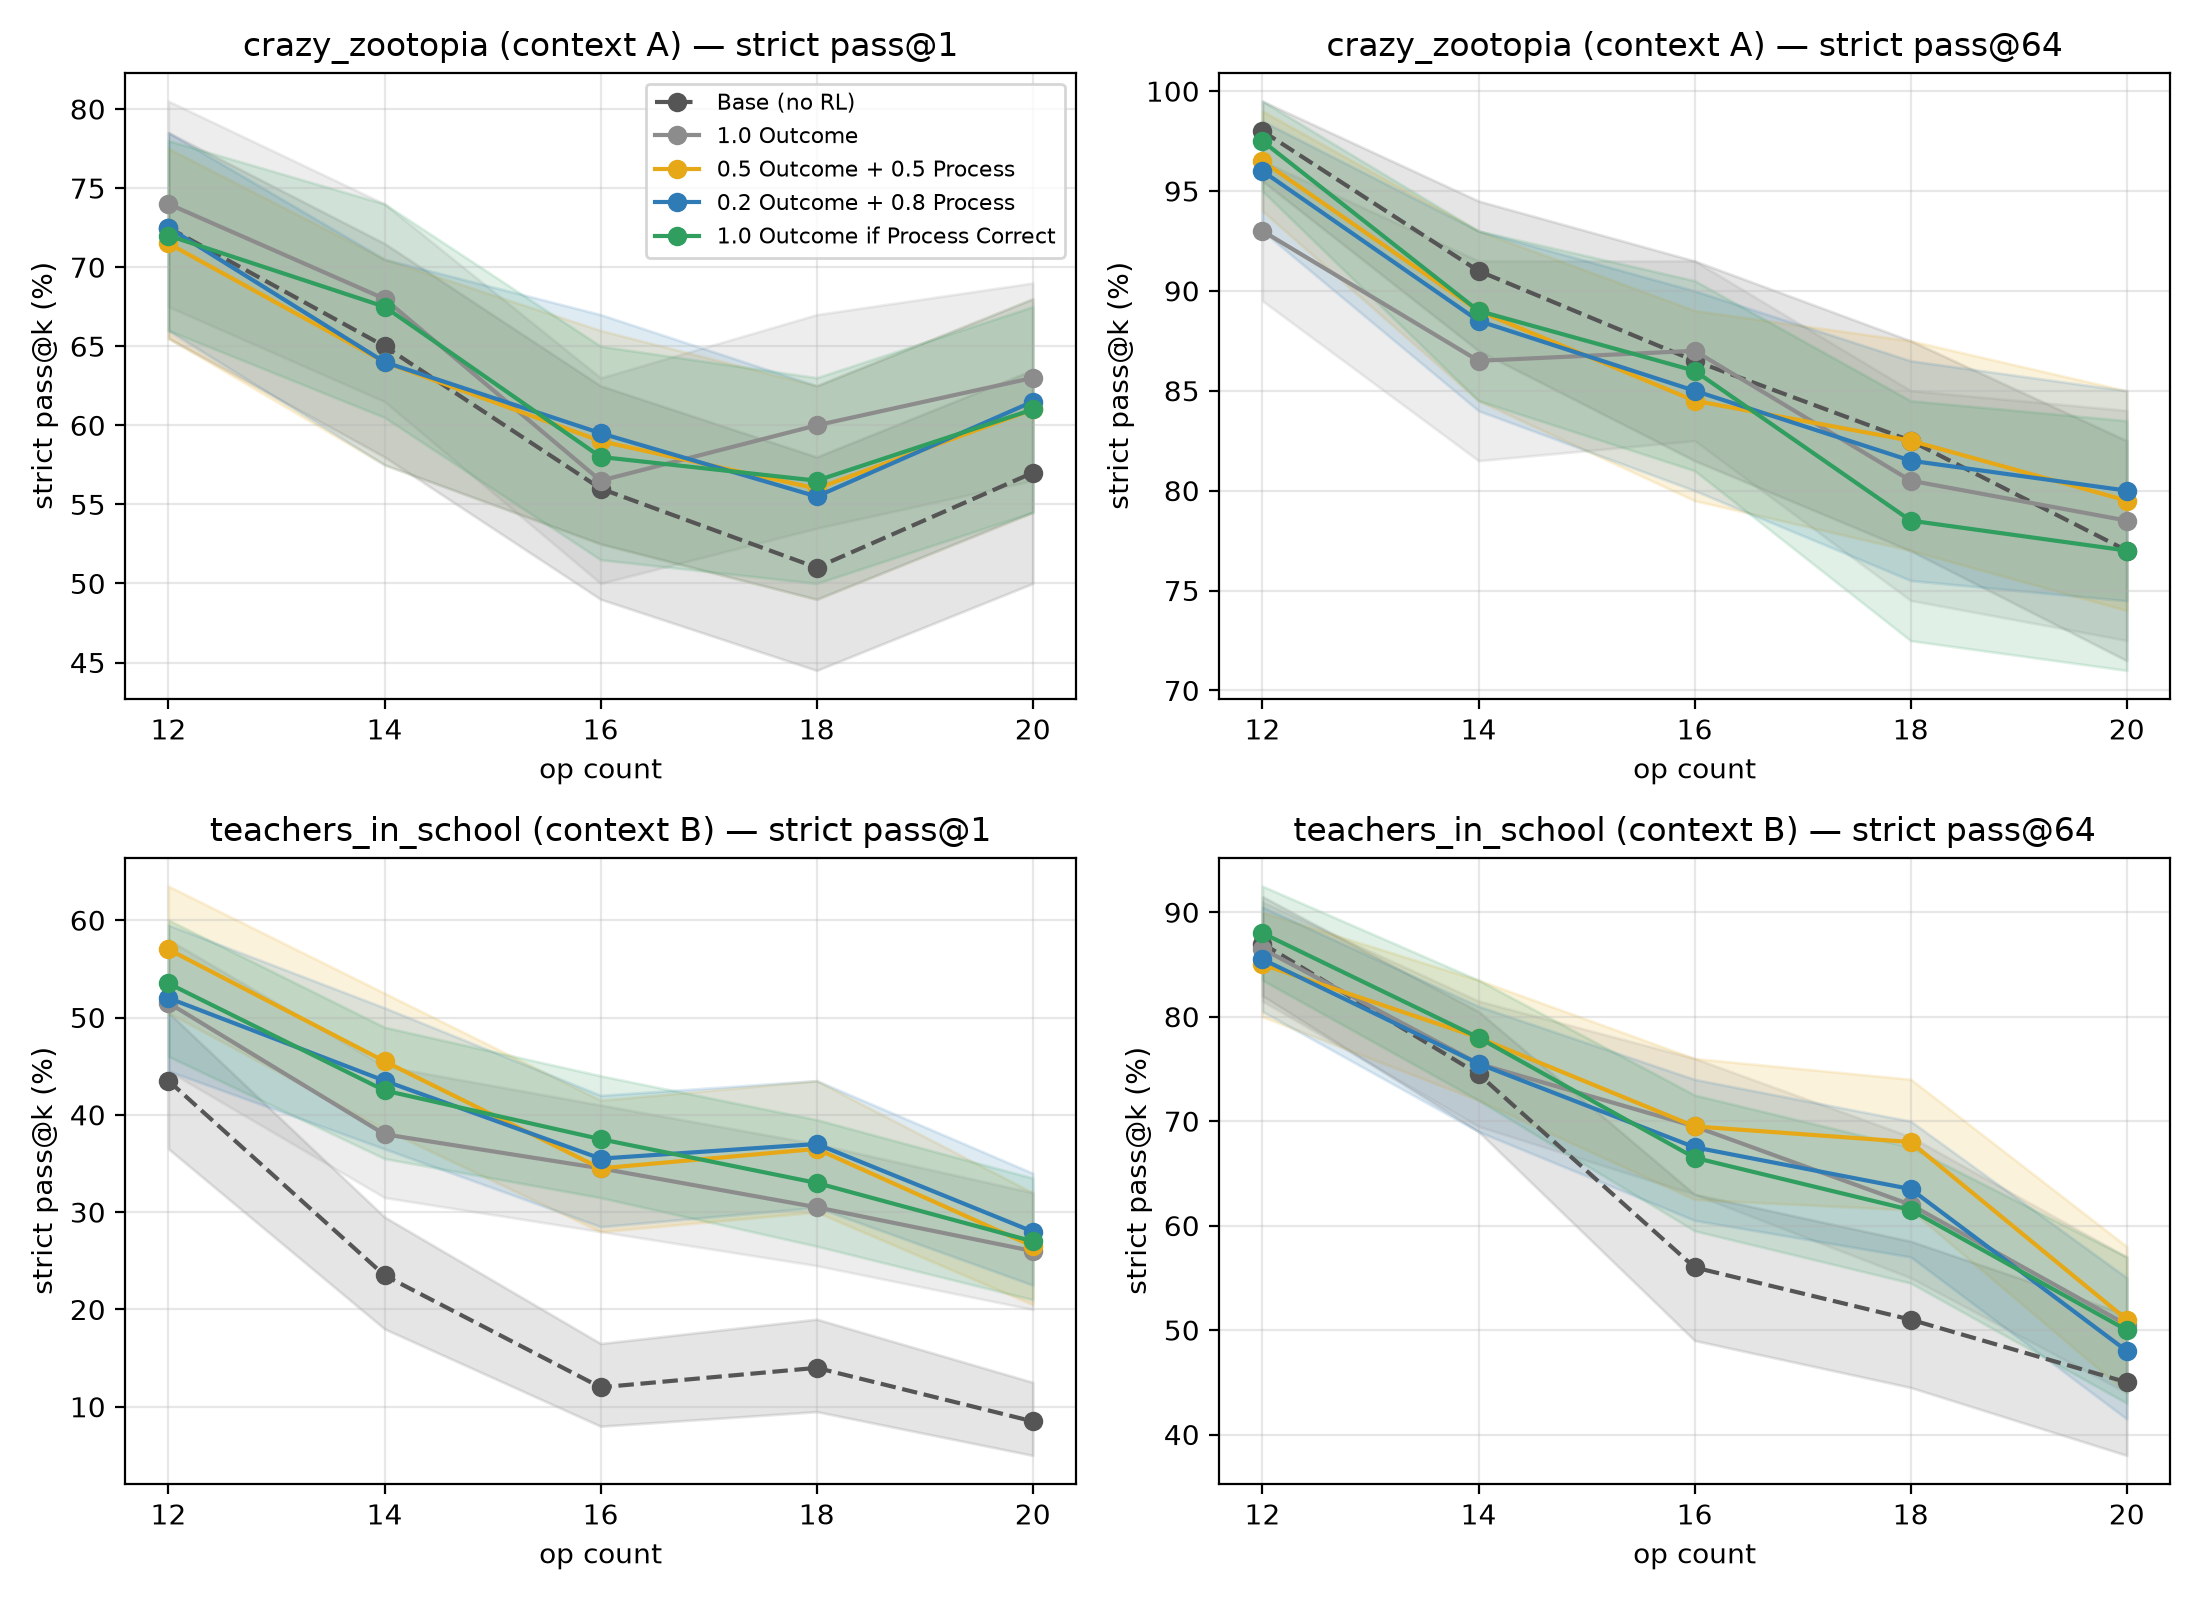
\includegraphics[width=\linewidth]{fig_passk_per_op.png}
\caption{Strict \passk{1} and \passk{64} per op count, both contexts, with $95\%$
bootstrap bands --- the full data behind the headline and per-op tables. The teachers
panels show RL lifting both \passk{1} and \passk{64} far above base (new ability on the
seeded long-tail context); the zoo panels show RL raising \passk{1} but not \passk{64}
(sharpening on already-covered material).}
\end{figure}

\begin{figure}[h]\centering
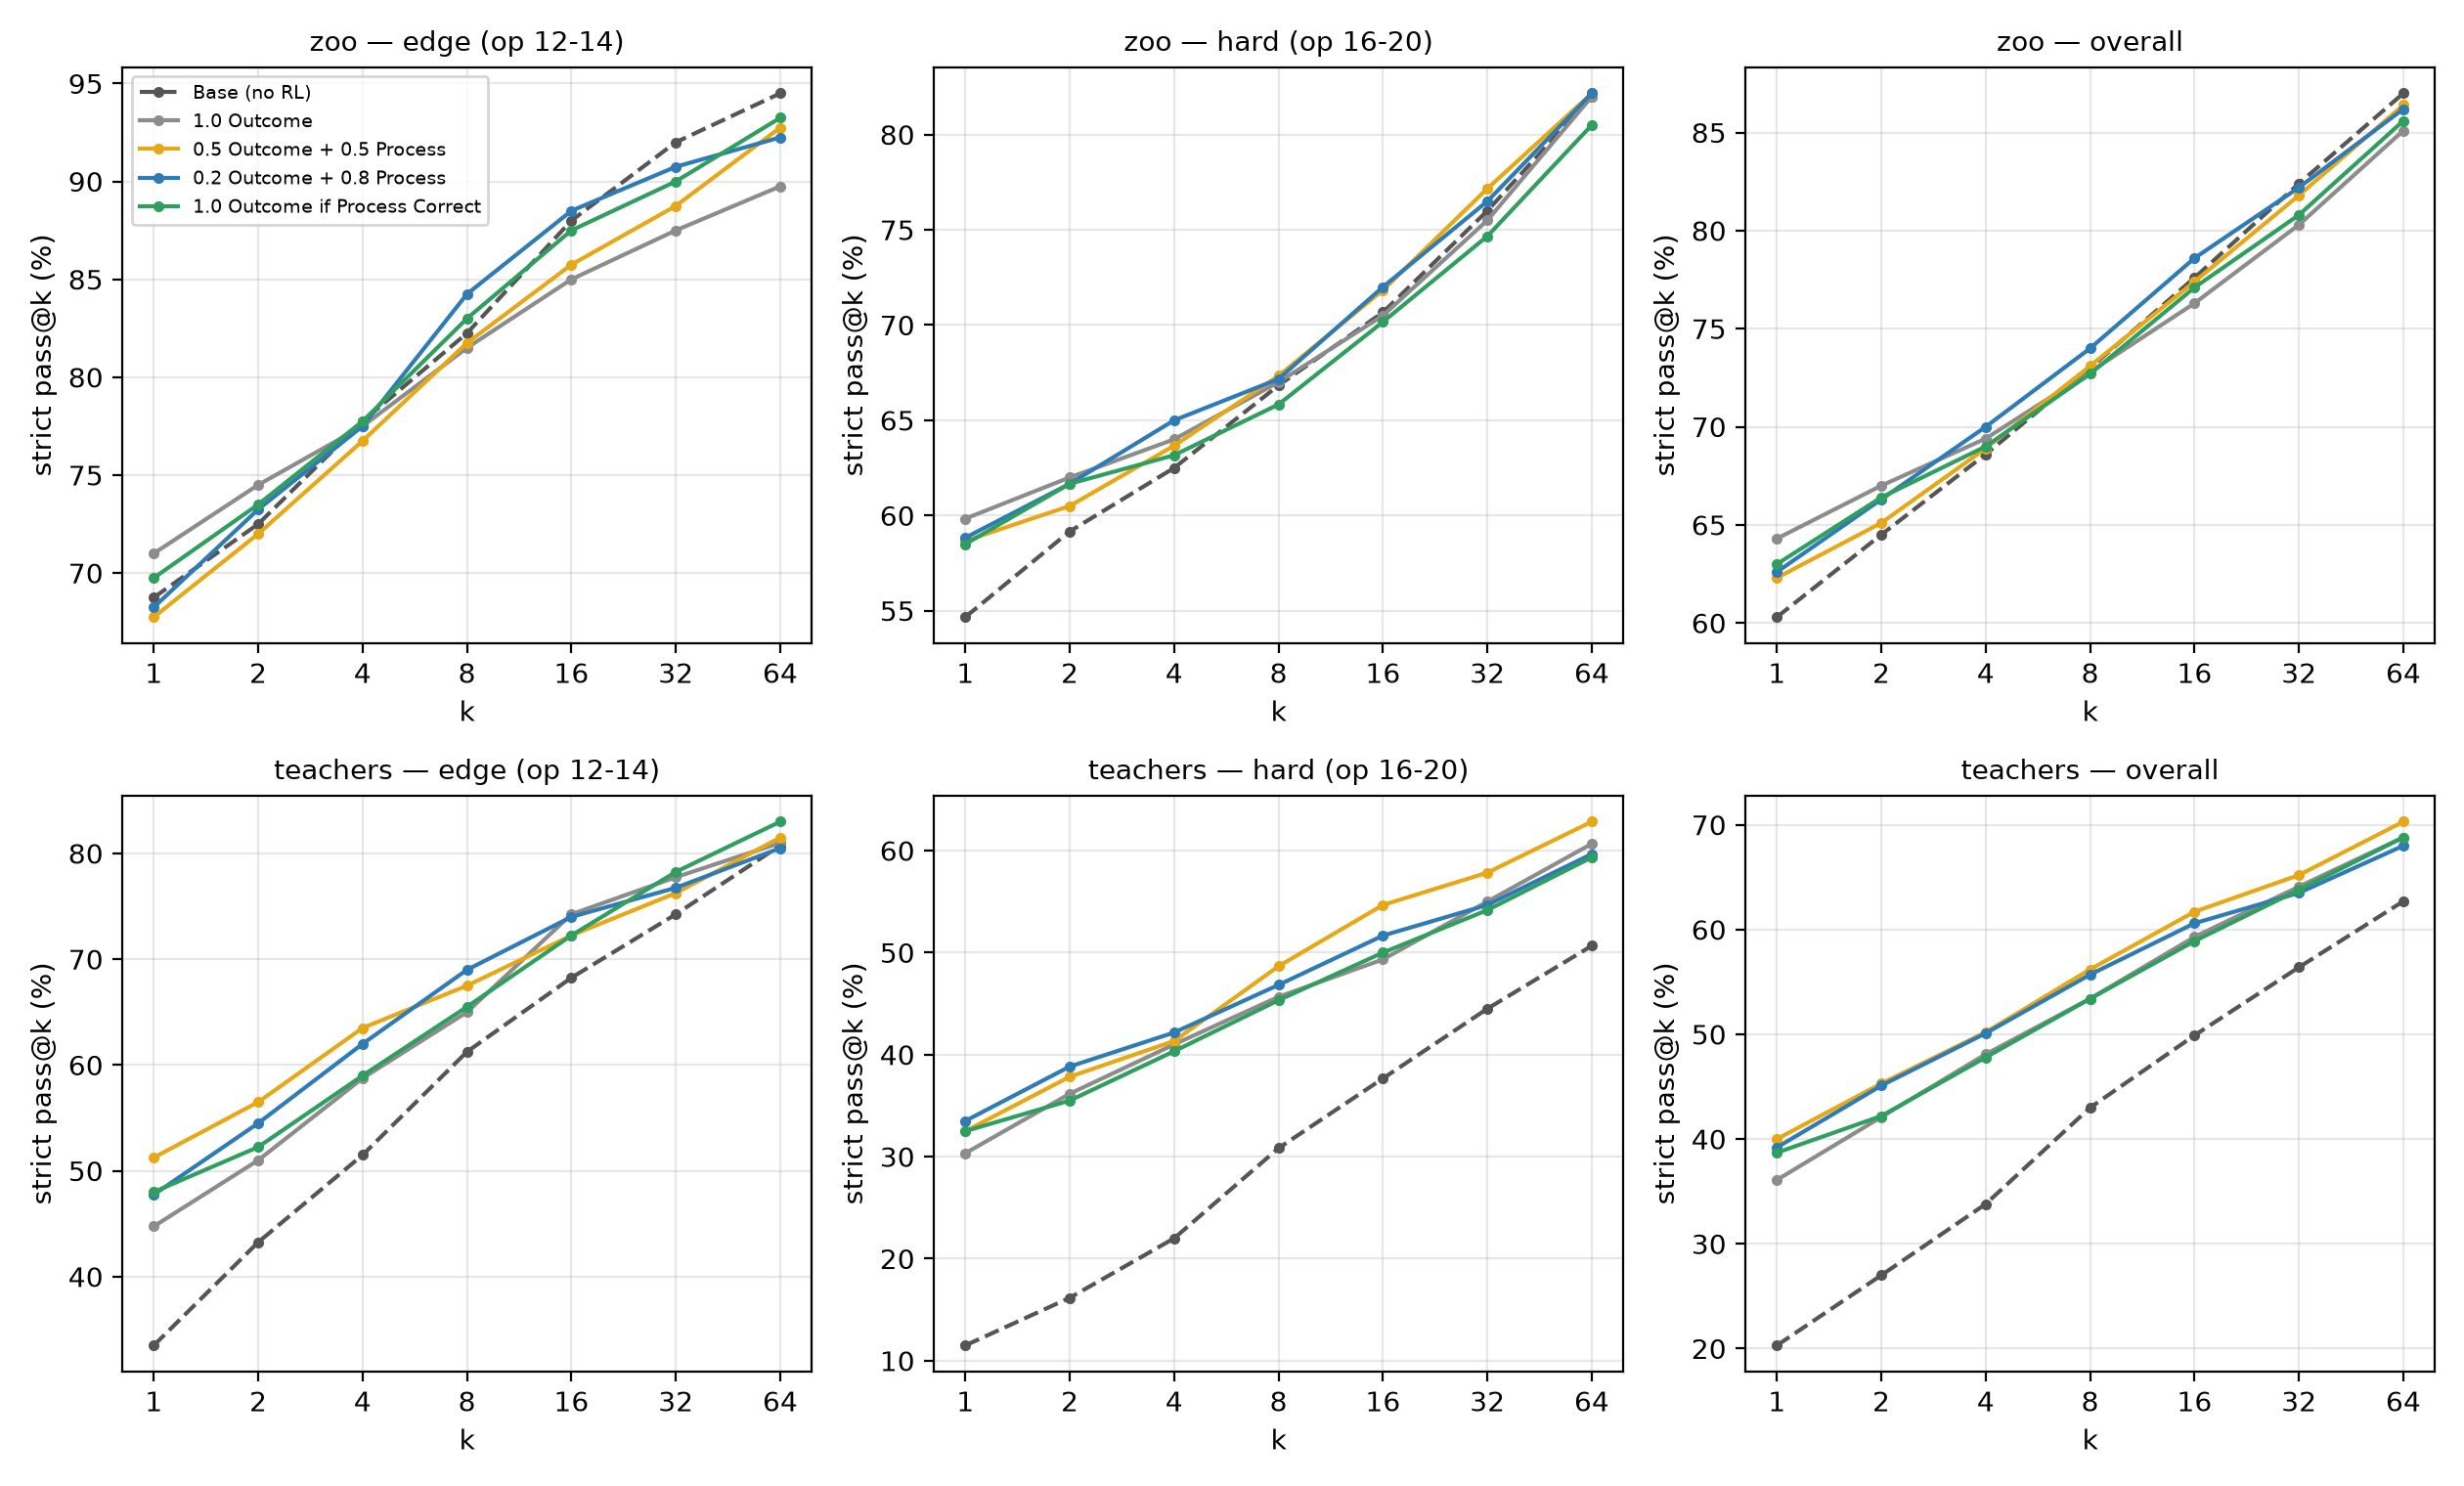
\includegraphics[width=\linewidth]{fig_passk_curves.png}
\caption{Strict \passk{k} vs.\ $k$ ($k=1\dots64$, log scale) per difficulty band and
overall, one line per reward. The gap between the base line and the RL lines on teachers,
and its near-closure on zoo at large $k$, visualize the sharpening-vs-new-ability
distinction.}
\end{figure}

\begin{figure}[h]\centering
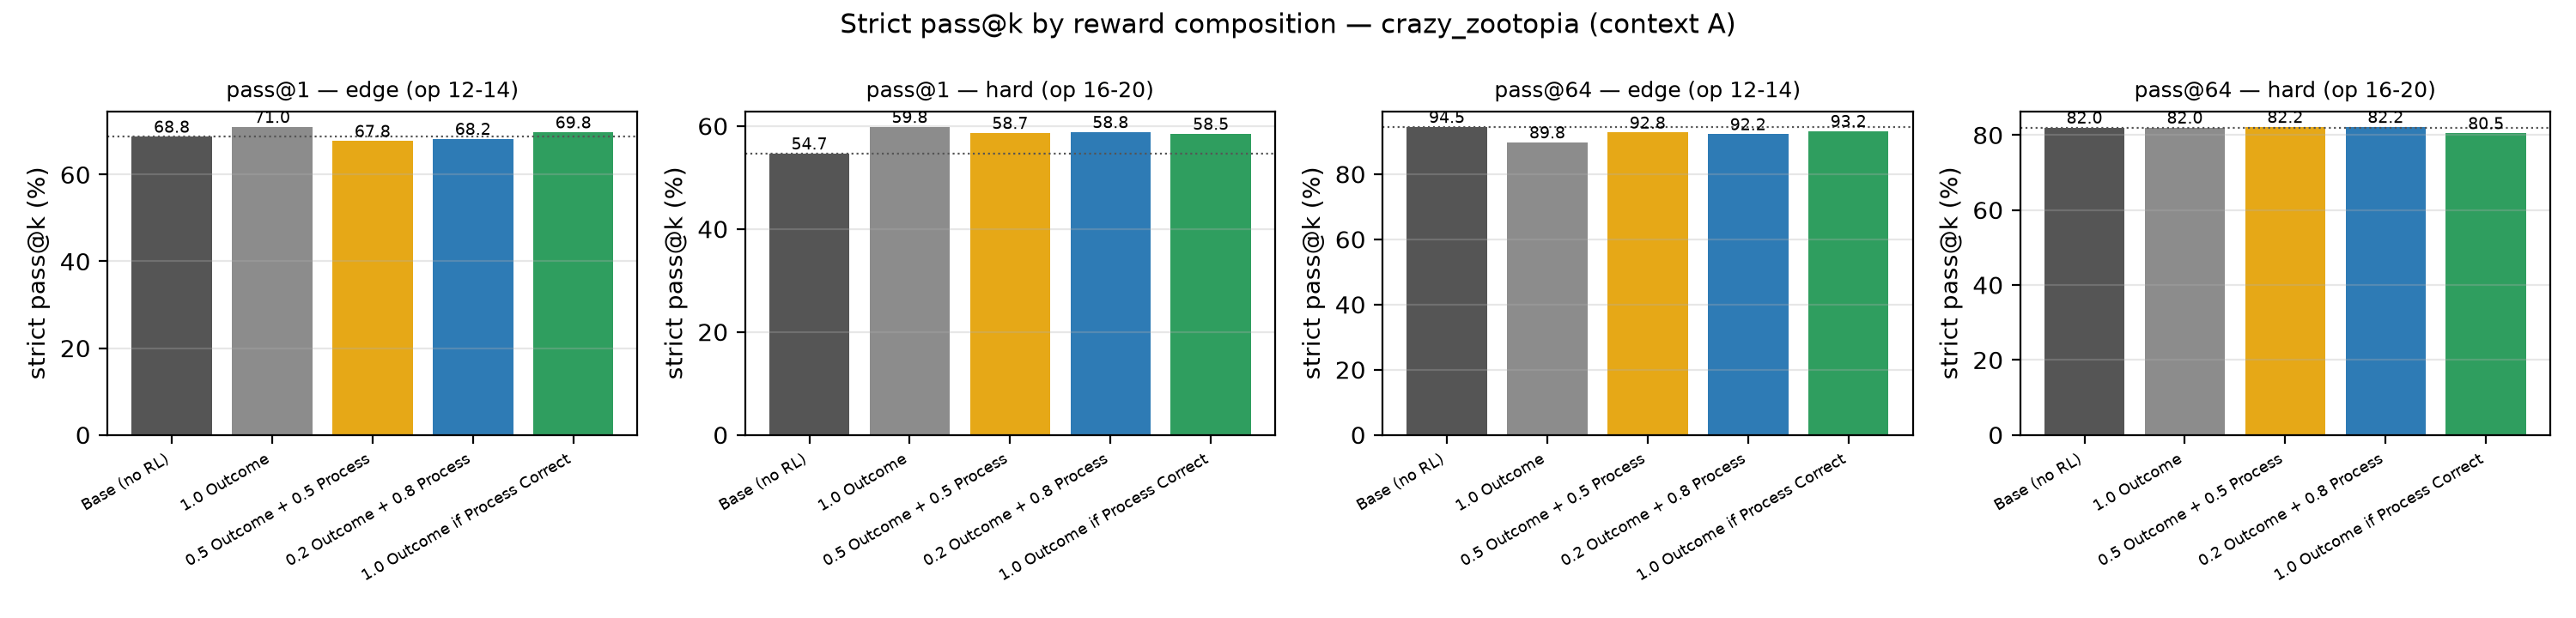
\includegraphics[width=.92\linewidth]{fig7_bars_zoo.png}
\caption{Strict \passk{1}/\passk{64} by reward composition and band, zoo context (the
well-covered context A). Contrast with the teachers bars in the main text: on zoo,
reward design barely moves the metrics --- process supervision matters most where the
model is weakest.}
\end{figure}

\begin{figure}[h]\centering
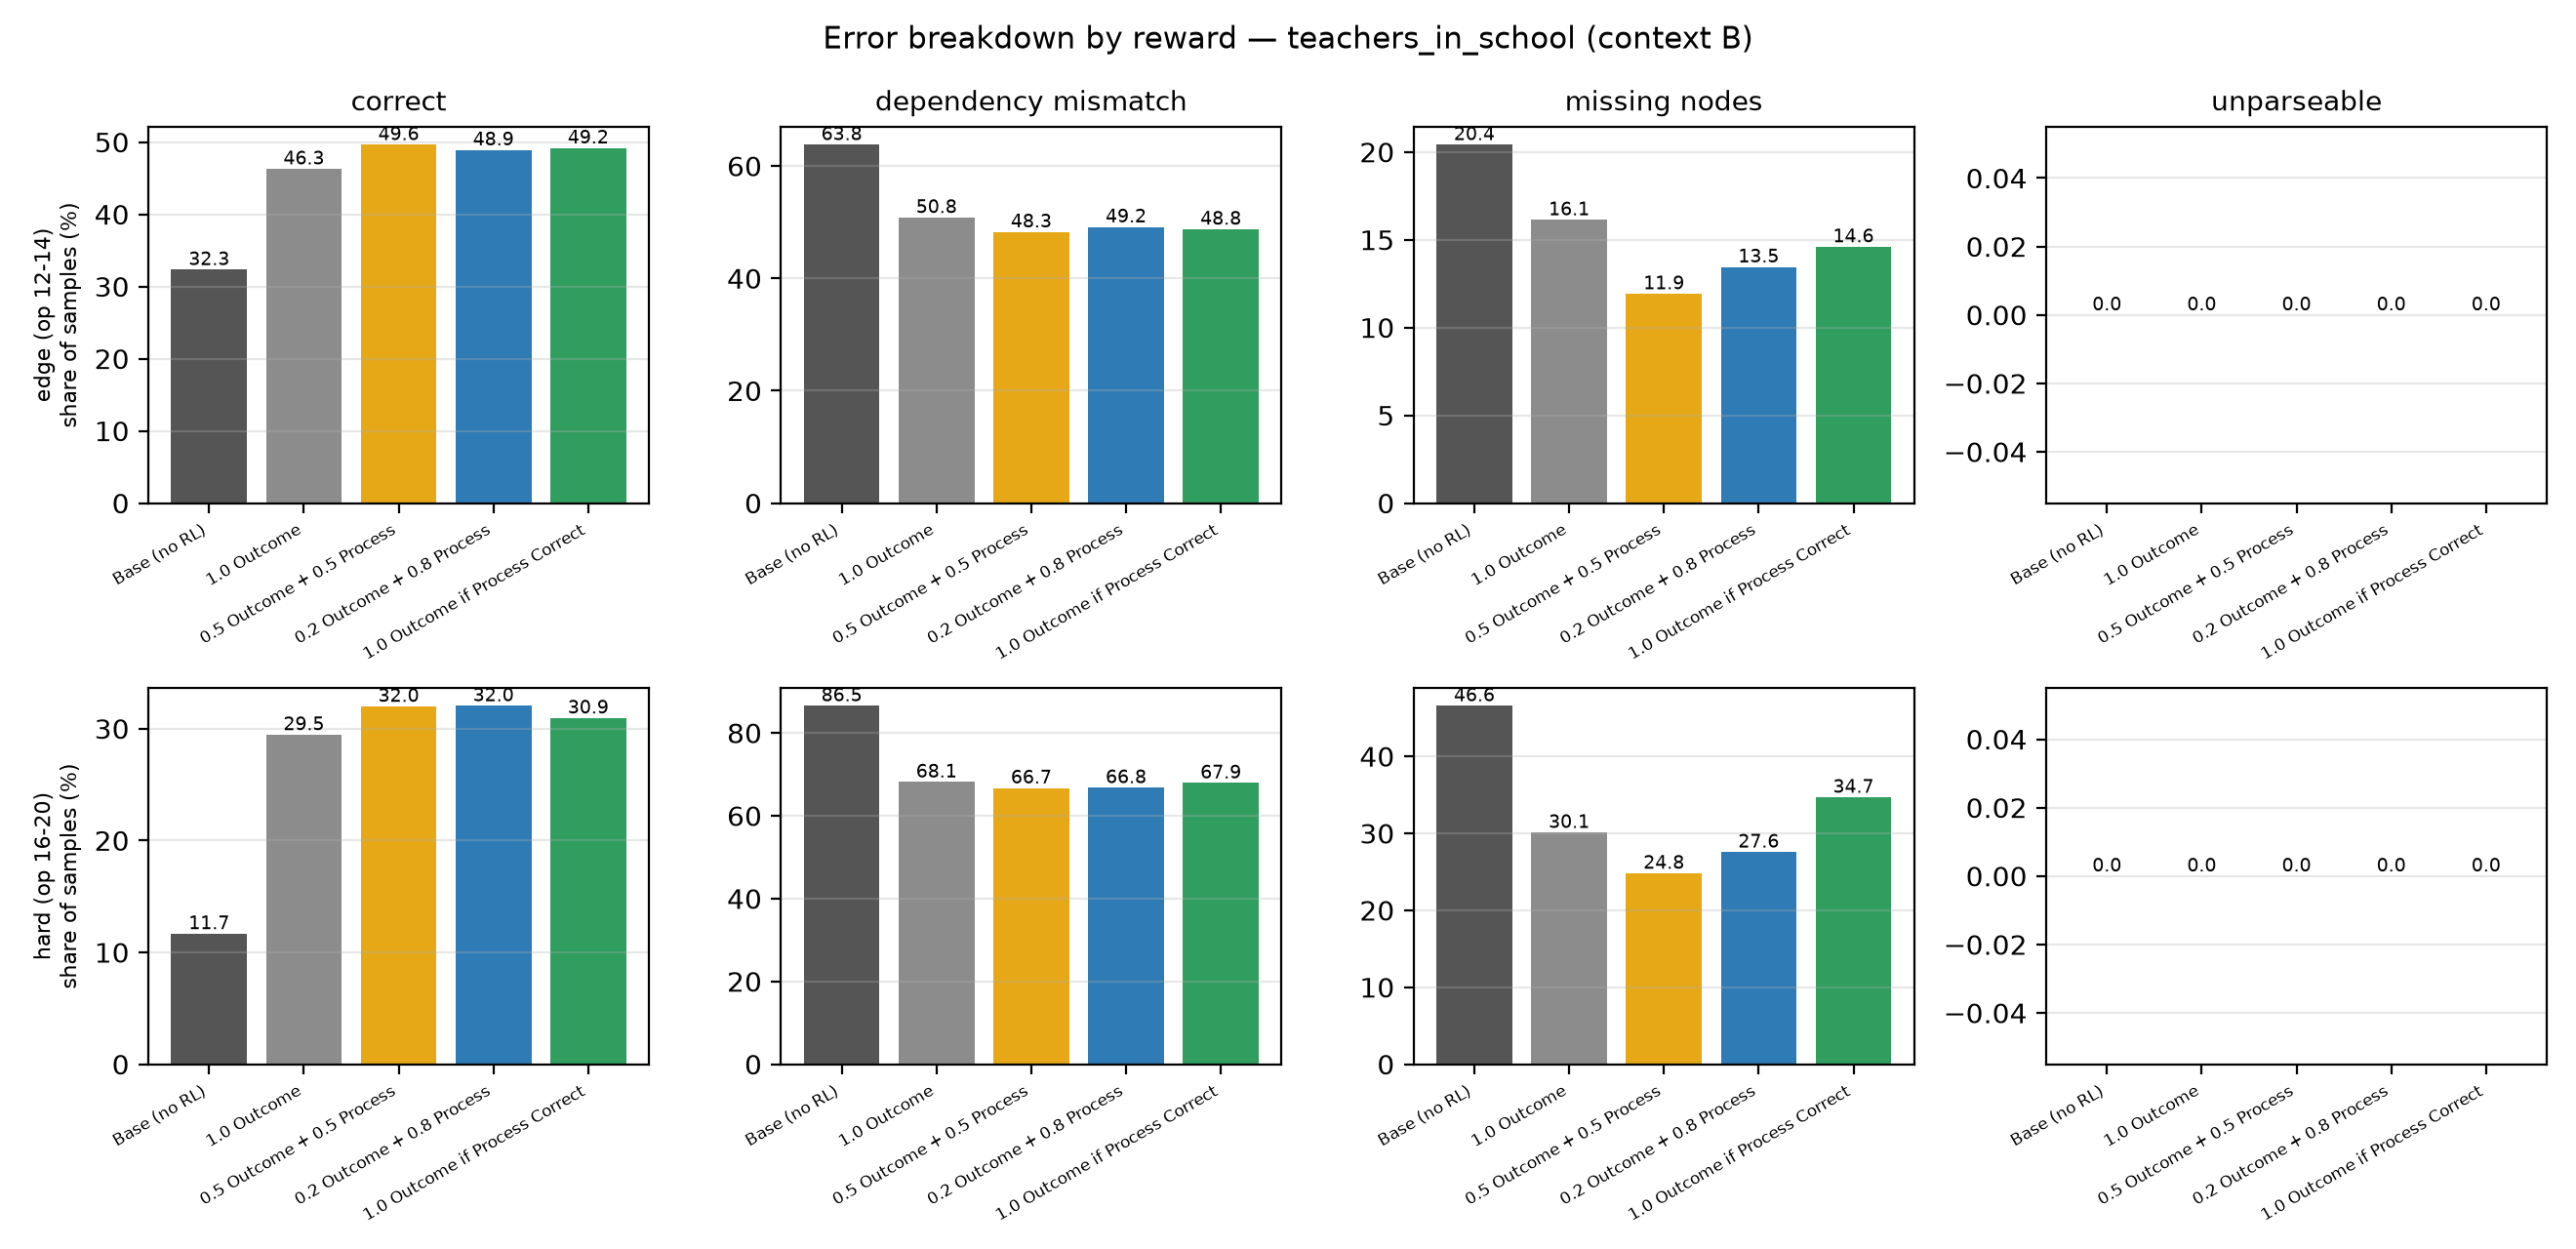
\includegraphics[width=\linewidth]{fig_error_breakdown_teachers.png}
\caption{Error-category shares by reward and band, teachers context (paper-Fig.-8
analogue). Process rewards shrink the wrong-dependency and missing-step shares; note the
strict-gating missing-step reversal on the hard band discussed in \S3.5.}
\end{figure}

\begin{figure}[h]\centering
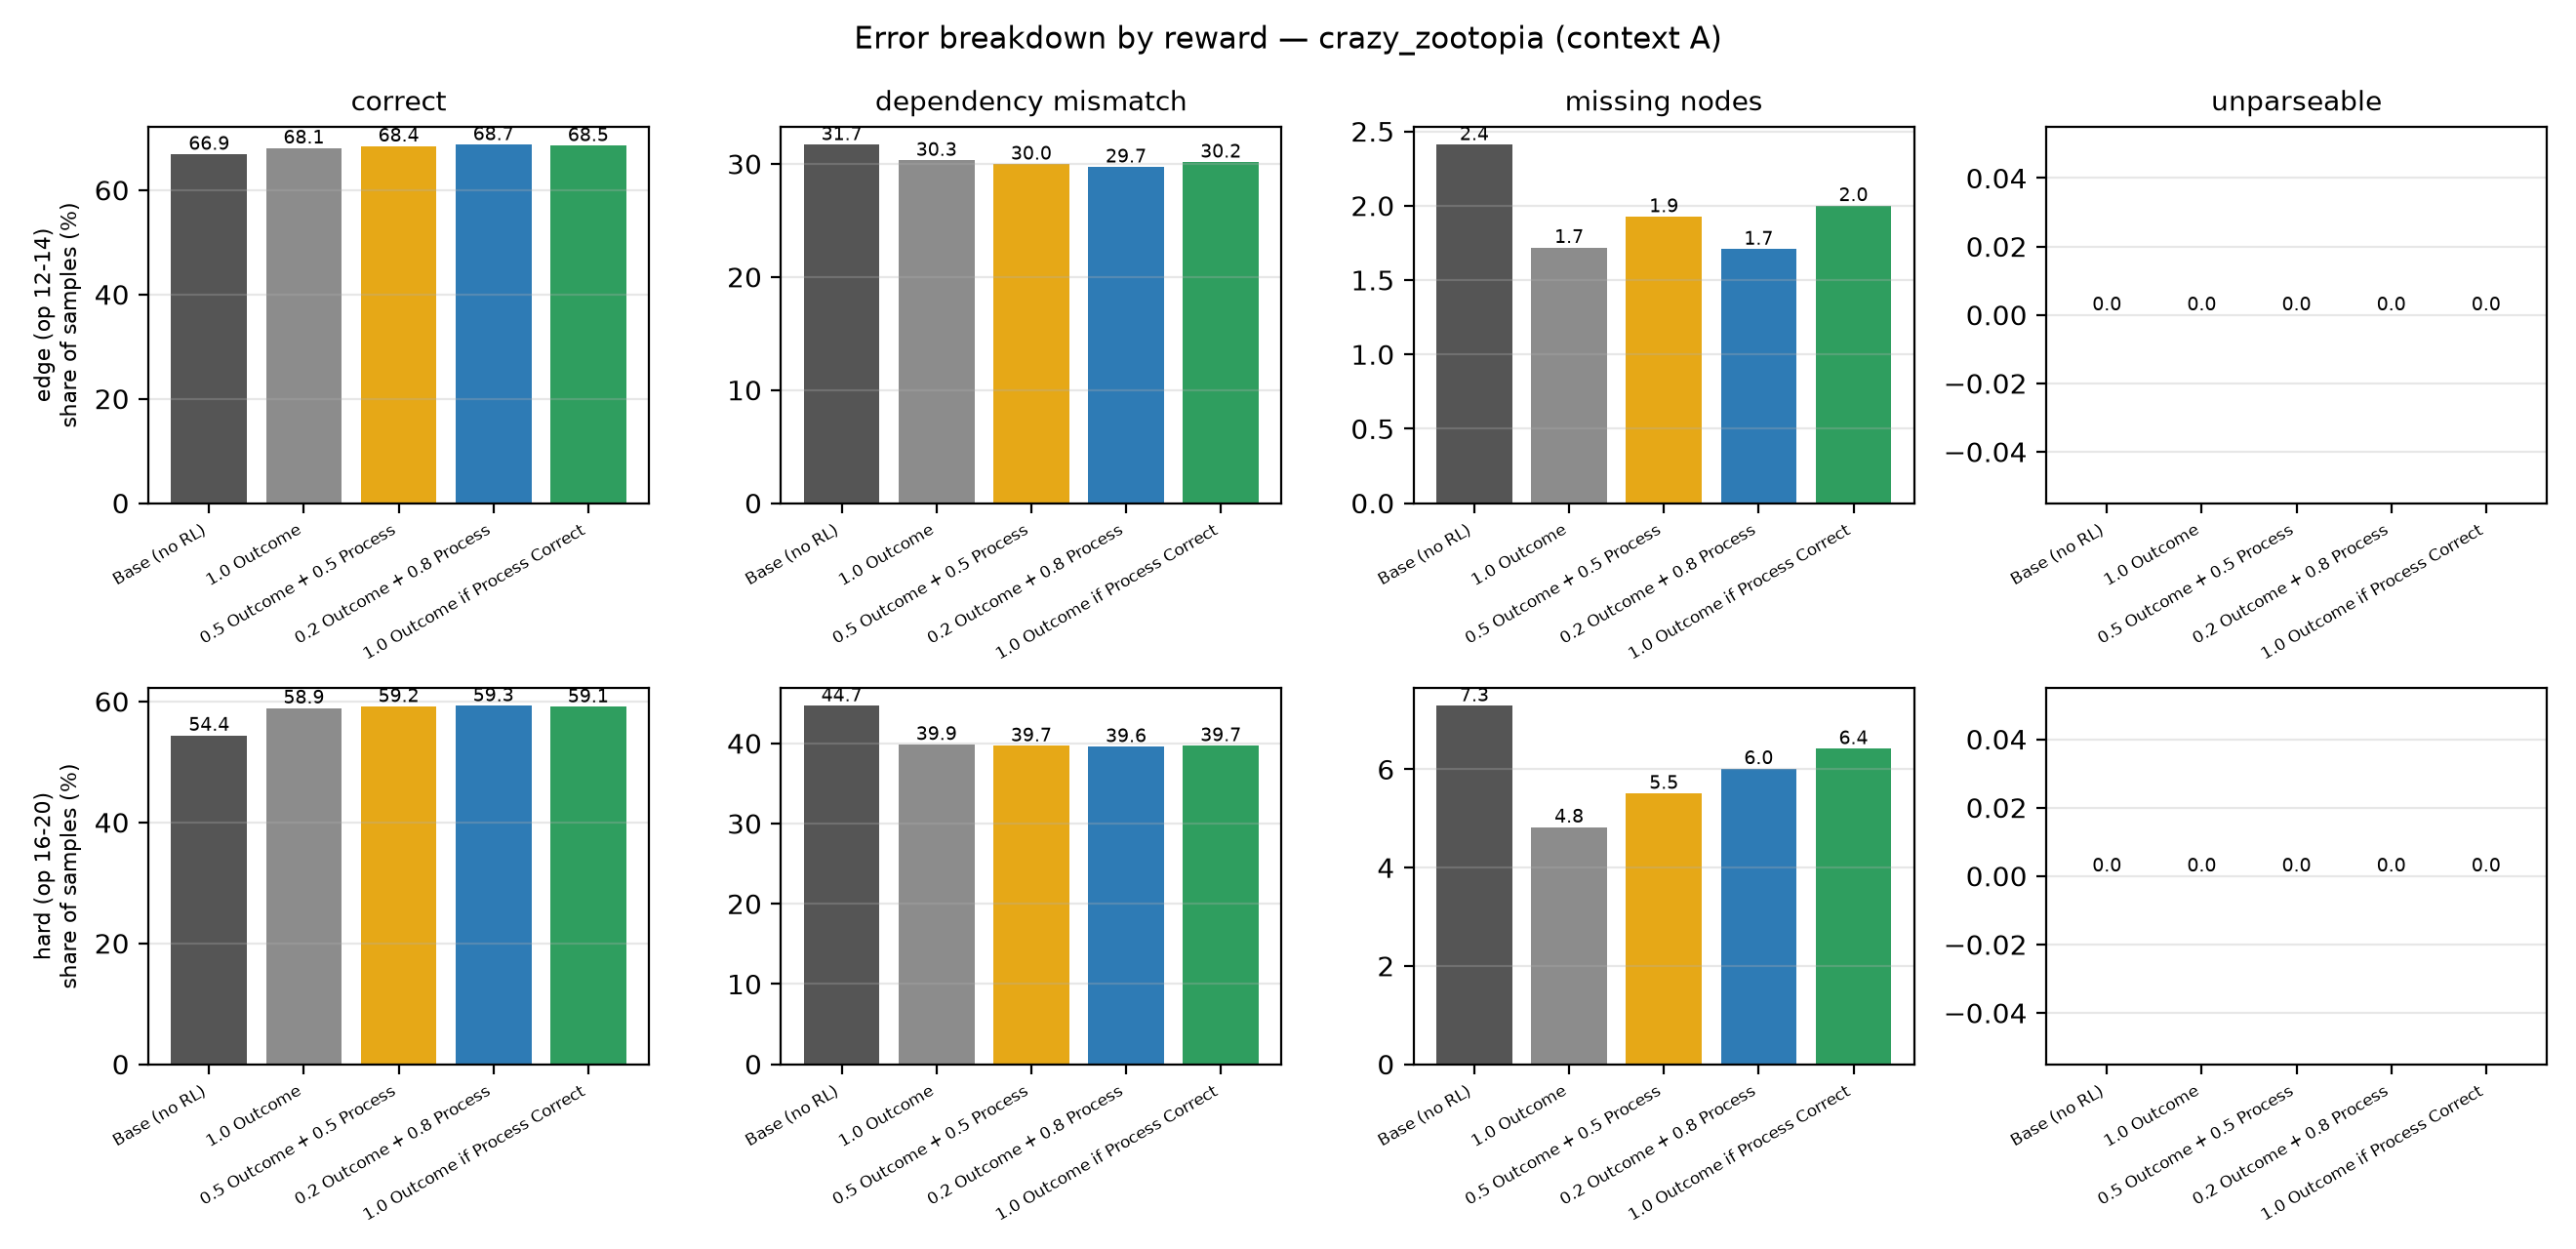
\includegraphics[width=\linewidth]{fig_error_breakdown_zoo.png}
\caption{Error-category shares by reward and band, zoo context --- shown for
completeness; the categories are largely saturated on this easy-for-the-model context.}
\end{figure}

\end{document}
